\documentclass[final]{cpecmu}

\projectNo{261492}
\acadyear{2025}
\titleTH{แพลตฟอร์มดิจิทัลสำหรับการค้นหาและวิเคราะห์รอยโรคก่อนมะเร็งและมะเร็งช่องปาก เฟส 2}
\titleEN{Digital Platform for Detecting and Analyzing Oral Potentially Malignant Disorders and Oral Cancer Phase 2}

\author{กวิน ชูสิน}{Kawin Choosin}{650610745}
\author{ณัฐพล ชนเวโรจน์}{Natthapon Chanawerot}{650612082}
\author{ธนวัฒน์ ใจเสริฐ}{Thanawat Jaisert}{650610768}
\author{ปริวัตร วงศ์อินทร์จันทร์}{Pariwat Wonginchan}{650612089}

\advisor{รศ.ดร.\,ปฏิเวธ วุฒิสารวัฒนา}{Assoc.\,Prof.\,Patiwet Wuttisarnwattana, Ph.D.}
\committee{ผศ.\,โดม โพธิกานนท์}{Asst.\,Prof.\,Dome Potikanond}
\committee{ผศ.ดร.\,นวดนย์ คุณเลิศกิจ}{Asst.\,Prof.\,Navadon Khunlertgit, Ph.D.}

\usepackage[final]{graphicx}
\usepackage{booktabs}
\usepackage{array}
\usepackage{tabularx}
\usepackage{colortbl}
\usepackage{enumitem}
\usepackage{float}
\usepackage{caption}
\usepackage{tcolorbox}
\tcbuselibrary{skins,breakable}
\usepackage{pifont}

\PassOptionsToPackage{hyphens}{url}
\usepackage[colorlinks=true,allcolors=Blue4,citecolor=red,linktoc=all]{hyperref}
\def\UrlLeft#1\UrlRight{$#1$}

\definecolor{primaryblue}{HTML}{1565C0}
\definecolor{lightblue}{HTML}{E3F2FD}
\definecolor{darkgray}{HTML}{212121}
\definecolor{medgray}{HTML}{757575}
\definecolor{successgreen}{HTML}{2E7D32}
\definecolor{phfill}{HTML}{F0F4FF}
\definecolor{phborder}{HTML}{90A4AE}
\definecolor{phtext}{HTML}{546E7A}
\definecolor{darkyellow}{HTML}{E65100}
\definecolor{dangerred}{HTML}{B71C1C}

\captionsetup{font=small, labelfont={bf,color=primaryblue}, skip=4pt}
\tcbset{
  bluebox/.style={enhanced,breakable,colback=lightblue,colframe=primaryblue,
    boxrule=1pt,arc=5pt,left=9pt,right=9pt,top=7pt,bottom=7pt,fonttitle=\bfseries},
  graybox/.style={enhanced,breakable,colback=gray!7,colframe=gray!35,
    boxrule=0.6pt,arc=5pt,left=9pt,right=9pt,top=7pt,bottom=7pt},
  greenbox/.style={enhanced,colback=green!6,colframe=successgreen,
    boxrule=0.8pt,arc=5pt,left=9pt,right=9pt,top=7pt,bottom=7pt},
  phbox/.style={enhanced,colback=phfill,colframe=phborder,
    boxrule=1pt,arc=4pt,left=10pt,right=10pt,top=16pt,bottom=16pt,
    halign=center,valign=center}
}

\newcommand{\placeholder}[2]{%
  \begin{tcolorbox}[phbox]
    {\color{phtext}\large\bfseries [\,ช่องว่างสำหรับรูปภาพ\,]}\\[5pt]
    {\color{primaryblue}\small\ttfamily #1}\\[5pt]
    {\color{phtext}\small #2}\\[6pt]
    {\color{medgray}\footnotesize\itshape แทนที่ด้วยไฟล์ภาพ: \texttt{#1}}
  \end{tcolorbox}%
}

\begin{document}
\maketitle
\makesignature

\ifproject
\begin{abstractTH}
โครงการนี้มีวัตถุประสงค์เพื่อพัฒนาแพลตฟอร์มดิจิทัลสำหรับการคัดกรองและวิเคราะห์รอยโรคก่อนมะเร็งและมะเร็งช่องปาก (Oral Potentially Malignant Disorders: OPMD และ Oral Cancer) โดยมุ่งเน้นการเพิ่มการเข้าถึงบริการทางทันตกรรมในกลุ่มผู้สูงอายุและประชาชนในพื้นที่ห่างไกล ระบบ eDENT-ELDER Phase 2 ได้รับการออกแบบให้เป็นแพลตฟอร์มแบบ Hybrid ที่ผสานเทคโนโลยีปัญญาประดิษฐ์ (AI) เข้ากับ Mobile Application และระบบ Tele-consult แบบ Asynchronous เพื่อสนับสนุนการคัดกรองโดยอาสาสมัครสาธารณสุขและบุคลากรแนวหน้า

ในด้านสถาปัตยกรรม ระบบได้รับการปรับปรุงจากรูปแบบ Monolithic ไปสู่ Modular Monolith บนแนวคิด Clean Architecture โดยใช้ Next.js สำหรับส่วน Frontend และ FastAPI สำหรับ Backend ร่วมกับฐานข้อมูล PostgreSQL และระบบจัดเก็บข้อมูล MinIO และ Redis เพื่อเพิ่มความสามารถในการขยายระบบและความทนทาน นอกจากนี้ ได้มีการพัฒนาระบบ AI แบบ Dual-Path ซึ่งประกอบด้วย Primary Path ที่ใช้ GPU (NVIDIA Triton Inference Server) และ Fallback Path ที่ใช้ CPU (TensorFlow Lite) เพื่อรองรับการทำงานต่อเนื่องและลดความเสี่ยงจาก Single Point of Failure โดยสามารถสลับการทำงานอัตโนมัติภายในเวลาไม่เกิน 1 วินาที

ผลการทดสอบระบบพบว่าสามารถรองรับการคัดกรองได้มากกว่า 500 กรณี โดยมีค่า latency เฉลี่ยต่ำกว่า 200 มิลลิวินาที และมีความเสถียรของระบบในระดับสูง นอกจากนี้ ระบบยังรองรับมาตรฐานความปลอดภัยของข้อมูล เช่น PDPA และ HIPAA ผ่านการเข้ารหัสแบบ End-to-End และการกำหนดสิทธิ์การเข้าถึงแบบ Role-Based Access Control

โดยสรุป ระบบ eDENT-ELDER Phase 2 เป็นแพลตฟอร์มทางการแพทย์ที่สามารถนำไปใช้งานจริงในระดับชุมชน ช่วยเพิ่มโอกาสในการตรวจพบโรคในระยะเริ่มต้น ลดภาระของบุคลากรทางการแพทย์ และสนับสนุนการพัฒนาระบบสุขภาพดิจิทัลอย่างยั่งยืน
\end{abstractTH}

\begin{abstract}
This project presents a digital platform for detecting and analyzing Oral Potentially Malignant Disorders (OPMD) and oral cancer, aiming to improve access to early screening among elderly populations and underserved communities. The proposed system, eDENT-ELDER Phase 2, is designed as a hybrid AI-driven medical platform integrating mobile applications and asynchronous teleconsultation to support frontline healthcare workers and village health volunteers.

The system architecture has been re-engineered from a monolithic design to a modular monolith based on Clean Architecture principles. It employs Next.js for the frontend and FastAPI for the backend, along with PostgreSQL, MinIO, and Redis for data management and processing. A key contribution is the Dual-Path AI system, which combines a GPU-based primary inference pipeline (NVIDIA Triton) with a CPU-based fallback (TensorFlow Lite), enabling automatic failover within one second and ensuring high system availability.

Experimental results demonstrate that the platform can process over 500 screening cases with an average inference latency below 200 ms and high system reliability. The platform also complies with medical data security standards, including PDPA and HIPAA, through end-to-end encryption and role-based access control.

In conclusion, eDENT-ELDER Phase 2 provides a scalable and reliable AI-assisted screening platform suitable for real-world deployment, enhancing early detection rates, reducing healthcare workload, and supporting sustainable digital health systems.
\end{abstract}

\iffalse
\begin{dedication}
This document is dedicated to all Chiang Mai University students.

Dedication page is optional.
\end{dedication}
\fi % \iffalse

\clearpage
\pagestyle{plain}
\chapter*{\ifenglish Acknowledgments\else กิตติกรรมประกาศ\fi}
\phantomsection
\addcontentsline{toc}{section}{\ifenglish Acknowledgments\else กิตติกรรมประกาศ\fi}

โครงการ “แพลตฟอร์มดิจิทัลสำหรับการค้นหาและวิเคราะห์รอยโรคก่อนมะเร็งและมะเร็งช่องปาก (eDENT-ELDER Phase 2)” 
สำเร็จลุล่วงไปได้ด้วยความกรุณาและการสนับสนุนจากหลายภาคส่วน

ขอกราบขอบพระคุณ รองศาสตราจารย์ ดร. ปฏิเวธ วุฒิสารวัฒนา 
(Assoc. Prof. Patiwet Wuttisarnwattana, Ph.D.) อาจารย์ที่ปรึกษา 
ที่ได้ให้คำแนะนำ ข้อเสนอแนะ และการสนับสนุนทางวิชาการอย่างใกล้ชิดตลอดระยะเวลาการดำเนินโครงการ 
รวมถึงช่วยชี้แนะแนวทางในการพัฒนาและปรับปรุงระบบให้มีประสิทธิภาพและเหมาะสมต่อการใช้งานจริง

ขอขอบพระคุณ ผู้ช่วยศาสตราจารย์ โดม โพธิกานนท์ 
(Asst. Prof. Dome Potikanond) และ ผู้ช่วยศาสตราจารย์ ดร. นวดนย์ คุณเลิศกิจ 
(Asst. Prof. Navadon Khunlertgit, Ph.D.) คณะกรรมการสอบ 
ที่ได้กรุณาให้คำแนะนำ ข้อคิดเห็น และข้อเสนอแนะอันเป็นประโยชน์

ขอขอบพระคุณคณาจารย์ ผู้เชี่ยวชาญ หน่วยงานที่เกี่ยวข้อง อาสาสมัครสาธารณสุข (อสม.) 
และบุคลากรทางการแพทย์ทุกท่าน ที่มีส่วนร่วมในการให้ข้อมูล ทดสอบระบบ 
และสนับสนุนการพัฒนาโครงการ

ขอขอบคุณเพื่อนร่วมทีมทุกคนที่ร่วมแรงร่วมใจในการออกแบบ พัฒนา และทดสอบระบบ 
จนโครงการสำเร็จลุล่วงตามเป้าหมาย

สุดท้ายนี้ ขอขอบคุณครอบครัวและผู้มีส่วนเกี่ยวข้องทุกท่าน 
ที่ให้การสนับสนุน กำลังใจ และความเข้าใจตลอดระยะเวลาการดำเนินโครงการ

คณะผู้จัดทำขอขอบพระคุณทุกท่านมา ณ โอกาสนี้

\acksign{2025}{3}{25}

\clearpage

\fi % \ifproject

\contentspage

\ifproject
\figurelistpage

\tablelistpage
\fi % \ifproject

% \abbrlist % this page is optional

% \symlist % this page is optional

% \preface % this section is optional


\pagestyle{empty}\cleardoublepage
\normalspacing \setcounter{page}{1} \pagenumbering{arabic} \pagestyle{cpecmu}

\chapter{\ifenglish Introduction\else บทนำ\fi}

\section{ที่มาและความสำคัญของปัญหา}

มะเร็งช่องปาก (Oral Cancer) ติดอันดับ 1 ใน 10 โรคที่พบบ่อยที่สุดในประเทศไทย
ความท้าทายสำคัญในชุมชนชนบทคือพฤติกรรมการซื้อยาปฏิชีวนะมารับประทานเองเมื่อมีแผลในช่องปาก
โดยไม่ปรึกษาแพทย์หรือทันตแพทย์ ส่งผลให้การวินิจฉัยล่าช้าและพบโรคในระยะลุกลาม
ทำให้ผลการรักษาแย่ลงอย่างมีนัยสำคัญ

%% >> แทนที่ด้วย: fig_bg_news.png
%% ที่มา: สไลด์ที่ 3 (ข่าว Amarin News)
\begin{figure}[H]
  \centering
  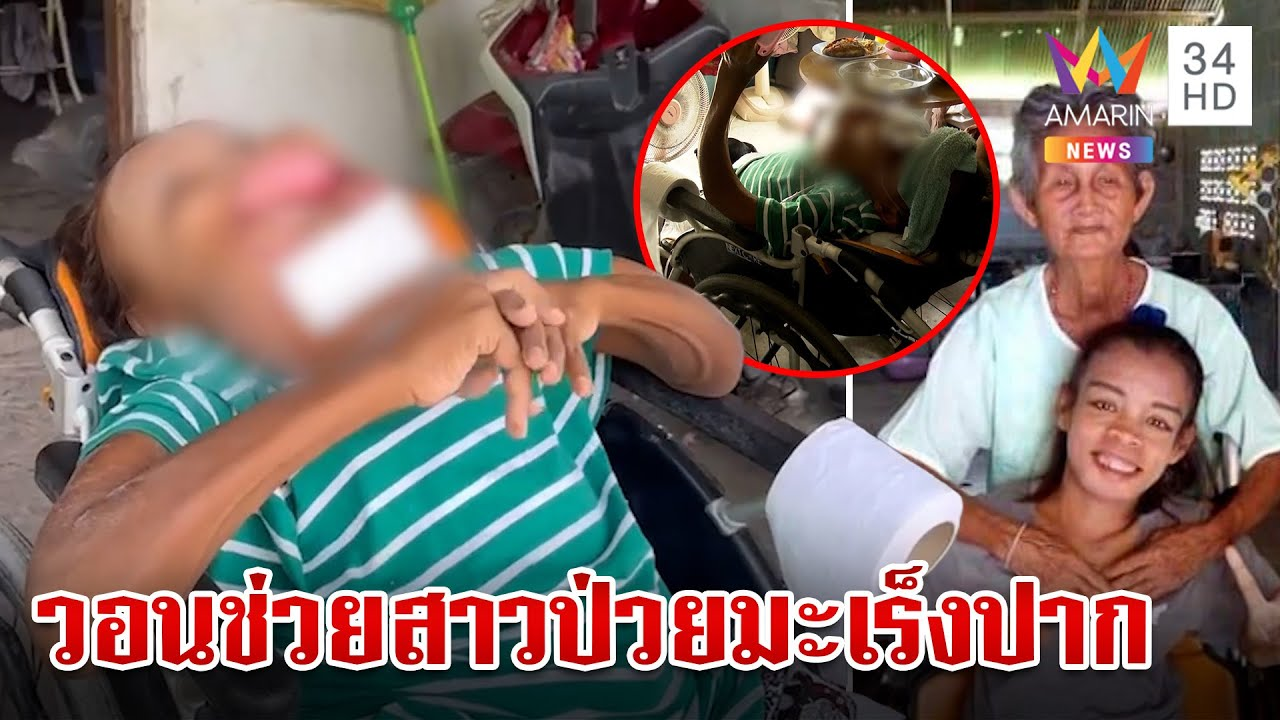
\includegraphics[width=0.9\linewidth]{fig/_bg/fig_bg_news.png}
  \caption{สื่อมวลชนรายงานปัญหาการวินิจฉัยมะเร็งช่องปากล่าช้า
    ผู้ป่วยในชนบทมักซื้อยามารับประทานเองจนอาการรุนแรง
    ที่มา: Amarin News / กรมอนามัย}
\end{figure}

ข้อมูลจากกรมอนามัย กระทรวงสาธารณสุข แบ่งรอยโรคในช่องปากออกเป็น 3 กลุ่มหลัก:

\begin{itemize}[leftmargin=1.8em, itemsep=3pt]
  \item \textbf{รอยโรคช่องปากทั่วไป (Oral Lesion)} --- พบมากที่สุด ครอบคลุมทุกช่วงอายุ
  \item \textbf{รอยโรคก่อนมะเร็ง (PMD --- Potentially Malignant Disorders)} ---
        รอยขาว (Leukoplakia) รอยแดง (Erythroplakia) ก้อน และแผลเล็กในช่องปาก
  \item \textbf{มะเร็งช่องปาก (OSCC --- Oral Squamous Cell Carcinoma)} ---
        พบมากในกลุ่มอายุ 60 ปีขึ้นไป
\end{itemize}

%% >> แทนที่ด้วย: fig_bg_lesion1.png และ fig_bg_lesion2.png
%% ที่มา: สไลด์ที่ 4
\begin{figure}[H]
  \centering
  \begin{minipage}[t]{0.48\linewidth}
    \centering
    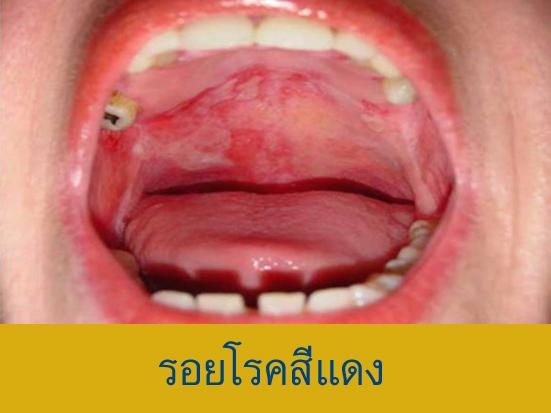
\includegraphics[width=\linewidth]{fig/_bg/fig_bg_lesion1.png}
    \caption{รอยโรคช่องปาก ตัวอย่างเคสที่ 1}
  \end{minipage}
  \hfill
  \begin{minipage}[t]{0.48\linewidth}
    \centering
    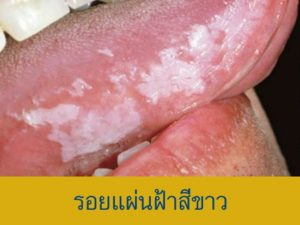
\includegraphics[width=\linewidth]{fig/_bg/fig_bg_lesion2.png}
    \caption{รอยโรคช่องปาก ตัวอย่างเคสที่ 2}
  \end{minipage}
\end{figure}

%% >> แทนที่ด้วย: fig_bg_lesion_annotated.png
%% ที่มา: สไลด์ที่ 5
\begin{figure}[H]
  \centering
  \begin{minipage}{0.65\linewidth}
    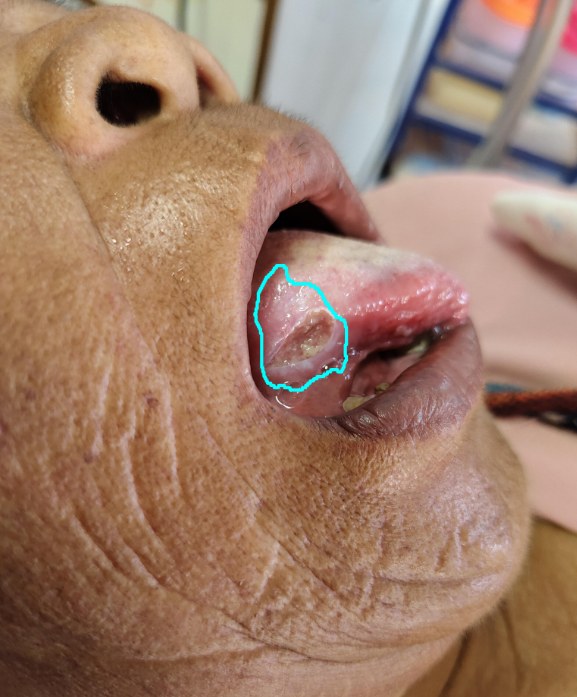
\includegraphics[width=\linewidth]{fig/_bg/fig_bg_lesion_annotated.png}
  \end{minipage}
  \caption{การ Annotation รอยโรคก่อนมะเร็งด้วย AI
    เส้นกรอบสีเหลืองแสดงบริเวณที่ส่งให้ผู้เชี่ยวชาญตรวจสอบ}
\end{figure}

%% >> แทนที่ด้วย: fig_bg_stats_chart.png
%% ที่มา: สไลด์ที่ 6
\begin{figure}[H]
  \centering
  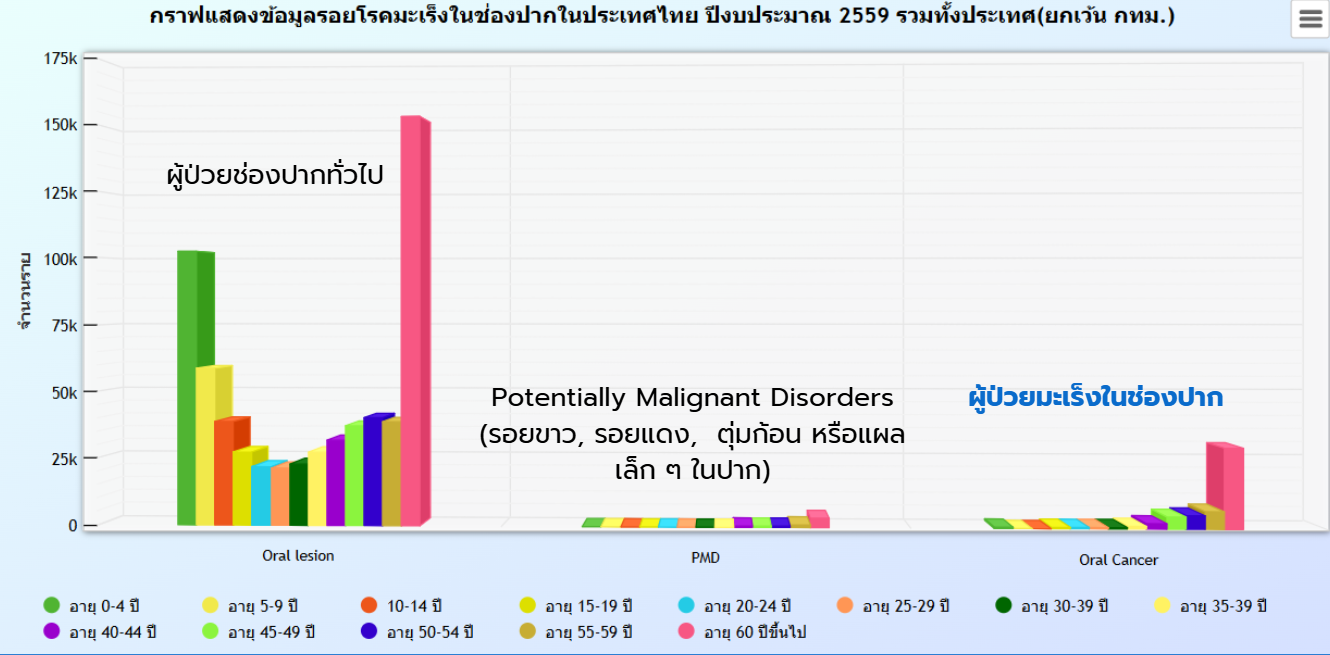
\includegraphics[width=0.95\linewidth]{fig/_bg/fig_bg_stats_chart.png}
  \caption{ข้อมูลรอยโรคช่องปากทั่วประเทศ ปีงบประมาณ 2559 (ยกเว้น กทม.)
    จำแนกเป็น 3 กลุ่ม ตามช่วงอายุ ที่มา: กรมอนามัย}
\end{figure}

%% >> แทนที่ด้วย: fig_bg_registry_table.png
%% ที่มา: สไลด์ที่ 7
\begin{figure}[H]
  \centering
  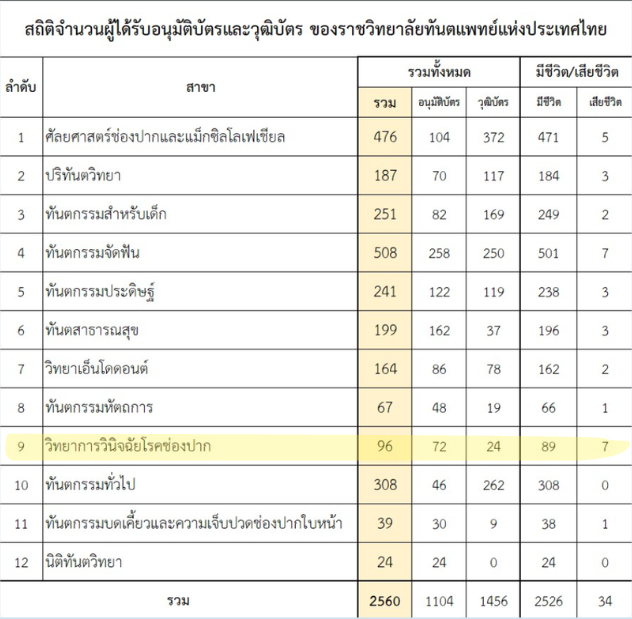
\includegraphics[width=0.95\linewidth]{fig/_bg/fig_bg_registry_table.png}
  \caption{จำนวนทันตแพทย์เฉพาะทาง ณ วันที่ 21 พฤศจิกายน 2567
    แถวที่ 9 (ไฮไลต์) สาขาวิทยาการวินิจัยโรคช่องปาก มีทันตแพทย์เพียง 96 คน}
\end{figure}

\begin{tcolorbox}[bluebox, title=ปัญหาหลัก]
  ผู้สูงอายุในชนบทอายุ 50 ปีขึ้นไป โดยเฉพาะกลุ่มเปราะบางที่พึ่งพาผู้ดูแล
  เผชิญอุปสรรคหนักในการเข้าถึงทันตแพทย์เฉพาะทาง
  เมื่อได้รับการวินิจฉัย มักพบว่าโรคลุกลามสู่ระยะท้ายแล้ว
  ส่งผลให้ผลการรักษาแย่ลงและค่าใช้จ่ายสูงขึ้นอย่างมาก
\end{tcolorbox}

\subsection{ข้อจำกัดทางเทคนิคของระบบเดิม}

แม้ระบบต้นแบบในเฟส~1 จะมีความแม่นยำของ AI ที่น่าพอใจ
แต่ยังไม่พร้อมสำหรับการใช้งานจริงในฐานะซอฟต์แวร์ทางการแพทย์
\textit{ในบริบทซอฟต์แวร์ทางการแพทย์ ความแม่นยำของ AI เพียงอย่างเดียวไม่เพียงพอ ---
ระบบต้องปลอดภัย โปร่งใส ตรวจสอบได้ และพร้อมใช้งานตลอดเวลา}
ระบบเดิมมีช่องโหว่สำคัญ 5 ประการ:

\begin{itemize}[leftmargin=1.8em, itemsep=4pt]
  \item \textbf{ไม่มีกรอบการปฏิบัติตาม PDPA / HIPAA} ---
        ข้อมูลสุขภาพผู้ป่วยถูกจัดเก็บโดยไม่ผ่านมาตรฐานคุ้มครองข้อมูลส่วนบุคคล
  \item \textbf{AI แบบ Monolith เป็น Single Point of Failure} ---
        หาก AI Service ล่ม ระบบทั้งหมดหยุดทำงานทันที ไม่มี Fallback
  \item \textbf{ไม่มีระบบ Audit Trail ป้องกันการแก้ไขย้อนหลัง} ---
        ไม่มีกลไกตรวจจับหรือป้องกันการแก้ไขเวชระเบียนย้อนหลัง
  \item \textbf{โค้ดแบบ Monolith ขยายระบบไม่ได้} ---
        การเปลี่ยนแปลงใดก็ตามเสี่ยงกระทบส่วนอื่น
        ไม่รองรับการ Scale Out แต่ละ Service
  \item \textbf{ไม่มี Role-Based Access Control (RBAC)} ---
        ผู้ใช้ทุกคนที่ผ่านการยืนยันตัวตนเข้าถึงข้อมูลและฟังก์ชันได้เหมือนกัน
\end{itemize}

\section{ระบบเดิม เฟส 1: AIDOC}

ระบบต้นแบบในเฟส~1 คือ \textbf{AIDOC}
(\textit{Artificial Intelligent System for Detecting and Analyzing PMDs and Oral Cancer})
พัฒนาและนำไปใช้งานร่วมกับกรมอนามัย
สร้างบน Flask Monolith Architecture ใช้ Bootstrap เป็น UI
จัดเก็บรูปภาพบน File System และใช้ MySQL เป็นฐานข้อมูล

%% >> แทนที่ด้วย: fig_aidoc_screenshot.png
%% ที่มา: สไลด์ที่ 8
\begin{figure}[H]
  \centering
  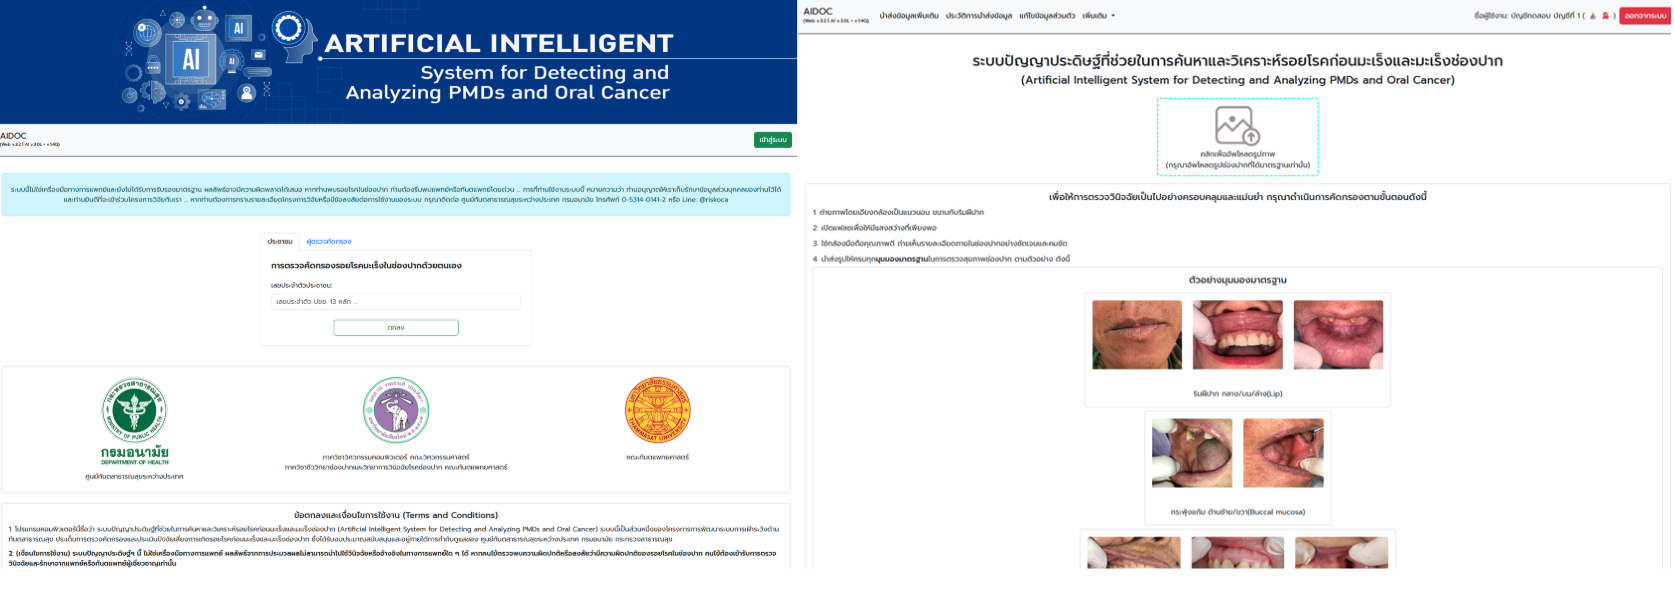
\includegraphics[width=0.95\linewidth]{fig/_bg/fig_aidoc_screenshot.png}
  \caption{ระบบ AIDOC เฟส 1: (ซ้าย) หน้า Consent และ Login;
    (ขวา) Workflow อัปโหลดภาพและคัดกรองด้วย AI
    สร้างด้วย Flask + Bootstrap + MySQL}
\end{figure}

\section{ข้อจำกัดของระบบเฟส 1}

\begin{tcolorbox}[bluebox]
  \centering\itshape
  ``ซอฟต์แวร์ทางการแพทย์ต้องมีความปลอดภัย โปร่งใส ตรวจสอบได้ และพร้อมใช้งานตลอดเวลา''
\end{tcolorbox}

%% >> แทนที่ด้วย: fig_legacy_arch.png
%% ที่มา: สไลด์ที่ 9 / 18
\begin{figure}[H]
  \centering
  \begin{minipage}{0.72\linewidth}
    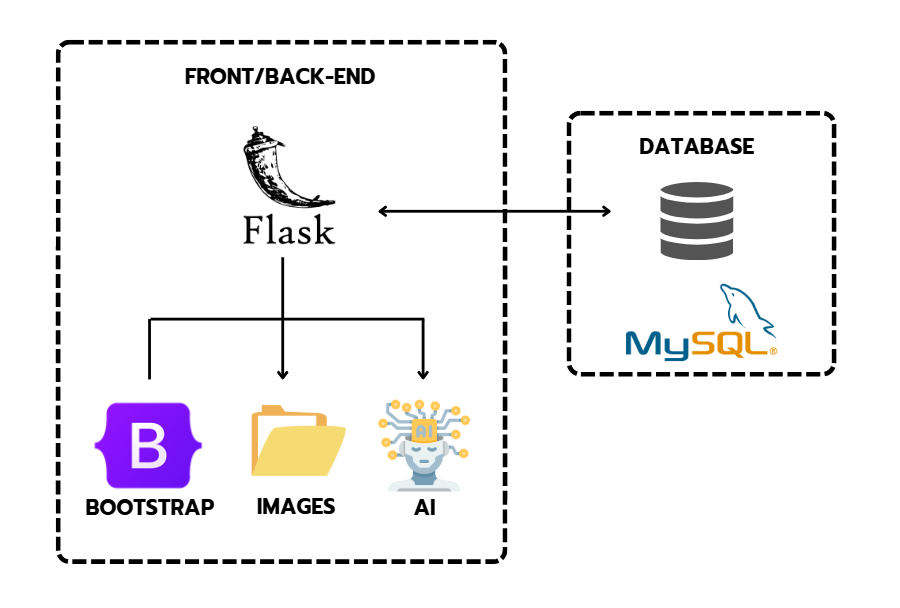
\includegraphics[width=\linewidth]{fig/_bg/fig_legacy_arch.png}
  \end{minipage}
  \caption{สถาปัตยกรรมระบบเดิม: Flask ทำหน้าที่ทั้ง Frontend, Backend, AI Inference
    และ Image Storage ในหน่วยเดียว ความล้มเหลวของส่วนใดทำให้ระบบทั้งหมดหยุด}
\end{figure}

\vspace{4pt}
\renewcommand{\arraystretch}{1.4}
\begin{tabularx}{\linewidth}{|>{\bfseries\color{primaryblue}}p{0.32\linewidth}|X|}
  \hline
  \rowcolor{primaryblue}
  \textcolor{white}{\textbf{ข้อจำกัด}} & \textcolor{white}{\textbf{ผลกระทบ}}\\
  \hline
  ไม่มีการปฏิบัติตาม PDPA / HIPAA &
    ข้อมูลผู้ป่วยขาดการคุ้มครองตามกฎหมายและข้อกำหนดที่เกี่ยวข้อง\\
  \hline
  Single Point of Failure &
    หาก Flask ล่ม ระบบทั้งหมดใช้งานไม่ได้ทันที\\
  \hline
  ไม่มี Audit Trail ป้องกันการแก้ไขย้อนหลัง &
    เวชระเบียนสามารถถูกแก้ไขโดยไม่มีหลักฐาน\\
  \hline
  โค้ดแบบ Monolith ขยายระบบยาก &
    การแก้ไข Bug หรืออัปเดต AI เสี่ยงทำให้ระบบอื่นพัง\\
  \hline
\end{tabularx}

\section{วิธีดำเนินงาน: การ Re-engineer สถาปัตยกรรมระบบ}

วิธีดำเนินงานหลักของเฟส~2 คือการ Re-engineer สถาปัตยกรรมระบบใหม่ทั้งหมด
โดยแบ่งออกเป็น 4 เสาหลักทางวิศวกรรม:

\subsection{เสาหลักที่ 1: Architecture Re-engineering}

\begin{itemize}[leftmargin=1.8em, itemsep=3pt]
  \item \textbf{Next.js} (Layered Design, Mobile-first) สำหรับ Frontend
        พร้อม Auth Guard และการแยก State Management
  \item \textbf{FastAPI + Clean Architecture + Domain-Driven Design (DDD)}
        สำหรับ Backend --- Business Logic แยกจาก AI Layer อย่างสมบูรณ์
  \item \textbf{Async Queue Processing} (Redis + Celery Workers)
        ขจัดปัญหาเว็บค้างและ API Timeout จาก Synchronous AI Inference
\end{itemize}

\subsection{เสาหลักที่ 2: High-Availability AI (Dual-Path Inference)}

\begin{itemize}[leftmargin=1.8em, itemsep=3pt]
  \item \textbf{Primary Path:} NVIDIA Triton Inference Server (GPU, gRPC)
        พร้อม TensorRT Optimization
  \item \textbf{Fallback Path:} TensorFlow Lite (CPU, HTTP)
        พร้อม Auto Failover อัตโนมัติ
  \item \textbf{Health Monitoring:} ตรวจสอบสถานะต่อเนื่อง
      เปิด Auto-Switch ภายในเวลาไม่เกิน $\leq 1\,\text{s}$
\end{itemize}

\subsection{เสาหลักที่ 3: Data and Processing Layer}

\begin{itemize}[leftmargin=1.8em, itemsep=3pt]
  \item \textbf{PostgreSQL} (OLTP + Audit) --- ฐานข้อมูลหลักพร้อม Immutable Audit Schema
  \item \textbf{Redis} --- Task Queue สำหรับงาน AI แบบ Async และ Cache
  \item \textbf{MinIO} --- Object Storage สำหรับรูปภาพทางคลินิก
  \item \textbf{Celery Workers} --- ประมวลผลเบื้องหลัง: AI Inference Queue,
        2-Tier Audit Chain, Archival และงาน Compliance
\end{itemize}

\subsection{เสาหลักที่ 4: Enterprise Security and Compliance}

\begin{itemize}[leftmargin=1.8em, itemsep=3pt]
  \item \textbf{TLS 1.3} เข้ารหัสการสื่อสารทุกส่วนแบบ End-to-End
  \item \textbf{Role-Based Access Control (RBAC)} ครอบคลุม 6 บทบาท:
        ผู้ป่วย, อสม., ทันตแพทย์, ผู้คัดกรอง, ผู้เชี่ยวชาญ, ผู้ดูแลระบบ
  \item \textbf{2-Tier Audit Logging + Hash-Chain} ป้องกันการแก้ไขย้อนหลัง
        ตรวจสอบได้ 100\%
  \item \textbf{PDPA / HIPAA-ready} สอดคล้องกับกฎหมายคุ้มครองข้อมูลส่วนบุคคลของไทย
\end{itemize}

\section{แนะนำ eDENT-ELDER เฟส 2}

\subsection{วิสัยทัศน์และคำขวัญ}

\begin{tcolorbox}[bluebox]
  \centering
  {\large\bfseries ``พบเร็ว \textendash{} ส่งต่อเร็ว \textendash{} ติดตามครบ''}\\[0.4em]
  \textit{``Detect Early \textemdash{} Refer Fast \textemdash{} Follow Up Completely''}
\end{tcolorbox}

\subsection{กลุ่มเป้าหมาย}

\begin{enumerate}[leftmargin=1.8em, label=\textbf{\arabic*.}, itemsep=4pt]
  \item \textbf{ผู้สูงอายุที่มีอายุ 50 ปีขึ้นไป} ---
        กลุ่มเปราะบาง อาศัยในชนบท และต้องพึ่งพาผู้ดูแล
  \item \textbf{บุคลากรสาธารณสุขแนวหน้า} ---
        อาสาสมัครสาธารณสุขประจำหมู่บ้าน (อสม.) ทันตาภิบาล
        และเจ้าหน้าที่ รพ.สต. ที่ผ่าน Train-the-Trainer 6--8 รุ่น
\end{enumerate}

\subsection{4 เสาหลักของแพลตฟอร์ม}

\begin{tcolorbox}[graybox]
  \renewcommand{\arraystretch}{1.5}
  \begin{tabularx}{\linewidth}{@{}>{\bfseries\color{primaryblue}}p{0.26\linewidth}X@{}}
    Hybrid Mobile Platform &
      อินเทอร์เฟซที่ใช้งานง่ายผ่านมุมมองมือถือ และ Web Dashboard
      สำหรับผู้ดูแลและเจ้าหน้าที่ภาคสนาม\\
    AI-Guided Screening &
      AI ตรวจจับรอยโรค OPMD/OSCC พร้อม Assisted-Capture
      และ Quality-Gate รับรองคุณภาพภาพถ่าย\\
    Elderly-Centric Empowerment &
      เสริมพลัง อสม. (อายุ 50+) ในการคัดกรอง
      สื่อสารความเสี่ยง และส่งต่ออย่างเป็นระบบ\\
    Asynchronous Teleconsultation &
      ระบบ Store-and-Forward เชื่อมต่อ อสม. กับผู้เชี่ยวชาญ
      โดยไม่ต้องนัดหมายพร้อมกัน\\
  \end{tabularx}
\end{tcolorbox}

\section{วัตถุประสงค์ของโครงงาน}

\begin{enumerate}[leftmargin=1.8em, label=\textbf{\arabic*.}, itemsep=6pt]
  \item \textbf{พัฒนาและทดสอบระบบ AI คัดกรอง} OPMD/OSCC ให้มีความแม่นยำสูง
    ใช้งานได้จริงในภาคสนาม และได้รับการยอมรับจากทันตแพทย์เฉพาะทาง
  \item \textbf{พัฒนาแพลตฟอร์ม eDENT-ELDER} รองรับการคัดกรองด้วยตัวเองและการคัดกรองชุมชน
  \item \textbf{ประเมินผลลัพธ์ด้านบริการและสังคม} วัดการเข้าถึง เวลาพบผู้เชี่ยวชาญ
        อัตราตรวจพบระยะแรก และความยั่งยืน
\end{enumerate}

\subsection{ประโยชน์ที่คาดว่าจะได้รับ}

\begin{itemize}[leftmargin=1.8em, itemsep=4pt]
  \item \textbf{ระดับระบบ:} แพลตฟอร์มที่ผสาน AI ปลอดภัย ตรวจสอบได้
        ลดภาระแนวหน้าและเพิ่มโอกาสตรวจพบระยะแรก (Stage-Shift)
  \item \textbf{ระดับชุมชน:} ผู้สูงอายุและครอบครัวในพื้นที่นำร่องได้รับการคัดกรองเร็วขึ้น
        หัวหน้า อสม. (อายุเฉลี่ย 50+) เป็นทั้งผู้ให้บริการและผู้รับประโยชน์
\end{itemize}

\begin{tcolorbox}[graybox]
  \textbf{พื้นที่นำร่องหลัก:}
  เชียงใหม่ \textbullet{} พะเยา \textbullet{} ภูเก็ต \textbullet{} หนองบัวลำภู\\
  \textbf{เครือข่ายเสริม:} สุรินทร์ สมุทรปราการ และจังหวัดอื่นตามความพร้อม
\end{tcolorbox}

\section{ภาคีและผู้ร่วมดำเนินงาน}

\renewcommand{\arraystretch}{1.3}
\begin{tabularx}{\linewidth}{lX}
  \toprule
  \textbf{หน่วยงาน} & \textbf{บทบาท}\\
  \midrule
  คณะทันตแพทยศาสตร์ มหาวิทยาลัยธรรมศาสตร์ &
    คำปรึกษาทางคลินิกและเครือข่ายผู้เชี่ยวชาญ\\
  คณะวิศวกรรมศาสตร์ มหาวิทยาลัยเชียงใหม่ &
    ทีมพัฒนาระบบ\\
  คณะทันตแพทยศาสตร์ มหาวิทยาลัยเชียงใหม่ &
    ตรวจสอบและให้ Feedback ทางคลินิก\\
  กรมอนามัย ศูนย์ทันตสาธารณสุขระหว่างประเทศ เชียงใหม่ &
    ความร่วมมือด้านข้อมูลและการ Deploy\\
  NurseCMU &
    บูรณาการงานสาธารณสุขชุมชน\\
  \bottomrule
\end{tabularx}


\chapter{\ifenglish System Workflow\else การทำงานของระบบ\fi}

\section{เครื่องมือคัดกรองสุขภาพช่องปาก}

\begin{tcolorbox}[bluebox]
  \textbf{Oral Health Assessment Tool (OHAT)} ---
  ประเมินสภาพช่องปากเพื่อคัดกรองความเสี่ยง
  และตัดสินใจว่าควรส่งภาพเข้า AI วิเคราะห์หรือไม่

  \vspace{0.5em}

  \textbf{Oral Health Impact Profile (OHIP)} ---
  ประเมินผลกระทบของสุขภาพช่องปากต่อคุณภาพชีวิต
  ทั้งความเจ็บปวด การใช้ชีวิตประจำวัน และการเข้าสังคม
\end{tcolorbox}

\section{กระบวนการยืนยันตัวตนและ Flow การทำงาน}

\subsection{ขั้นตอนการยืนยันตัวตน}

\begin{enumerate}[leftmargin=1.8em, itemsep=3pt]
  \item ผู้ใช้งานกรอกหมายเลขโทรศัพท์
  \item ระบบตรวจสอบสถานะการลงทะเบียนในทะเบียนราษฎร์
  \item \textit{กรณีผู้ใช้ใหม่:} ลงทะเบียน Consent ตาม PDPA และยืนยันบทบาท
  \item ส่งและยืนยัน OTP ผ่าน SMS
  \item ให้สิทธิ์ตามบทบาท (ผู้ป่วย หรือ อสม./ผู้คัดกรอง)
\end{enumerate}

%% >> แทนที่ด้วย: fig_auth_flow.png
%% ที่มา: สไลด์ที่ 12
\begin{figure}[H]
  \centering
  \placeholder{fig\_auth\_flow.png}{Diagram Flow การยืนยันตัวตน พร้อมภาพหน้าจอ Mobile (สไลด์ 12)}
  \caption{ขั้นตอนการยืนยันตัวตนของ eDENT-ELDER:
    กรอกเบอร์โทร ยืนยัน OTP ลง Consent PDPA และได้รับสิทธิ์ตามบทบาท}
\end{figure}

\subsection{Flow การทำงานระบบแบบ 5 เลน}

\renewcommand{\arraystretch}{1.4}
\begin{tabularx}{\linewidth}{|l|X|}
  \hline
  \rowcolor{primaryblue}
  \textcolor{white}{\textbf{เลน}} & \textcolor{white}{\textbf{หน้าที่}}\\
  \hline
  \textbf{เลน 1} \textemdash{} ผู้ป่วย / อสม. &
    รับข้อมูลและ Consent; แบบสอบถาม OHAT/OHIP;
    ถ่ายภาพผ่าน Quality Gate; ส่งเข้า AI\\
  \hline
  \textbf{เลน 2} \textemdash{} ระบบ AI &
    ตรวจสอบคุณภาพภาพ; ตรวจจับรอยโรคและประเมินความเสี่ยง;
    จัดการ Fallback\\
  \hline
  \textbf{เลน 3} \textemdash{} ผู้คัดกรอง &
    Screener Dashboard; Triage ผล AI;
    Flag Retrain หรือ Escalate\\
  \hline
  \textbf{เลน 4} \textemdash{} ผู้เชี่ยวชาญ &
    ยืนยันวินิจฉัย; แจ้งเตือน LINE; ติดตาม 14 วัน; ปิดเคส\\
  \hline
  \textbf{เลน 5} \textemdash{} ผู้ดูแลระบบ / วิชาการ &
    Dashboard ระดับประชากร; แผนที่ความเสี่ยงจังหวัด; กำกับระบบ\\
  \hline
\end{tabularx}

\vspace{8pt}

%% >> แทนที่ด้วย: fig_system_flow.png
%% ที่มา: สไลด์ที่ 13
\begin{figure}[H]
  \centering
  \placeholder{fig\_system\_flow.png}{Diagram Flow 5 เลนพร้อมภาพหน้าจอทุกกลุ่มผู้ใช้ (สไลด์ 13)}
  \caption{Flow การทำงานระบบ eDENT-ELDER แบบ 5 เลน}
\end{figure}

\subsection{อินเทอร์เฟซ Mobile สำหรับผู้ป่วยและ อสม.}

%% >> แทนที่ด้วย: fig_patient_vhv_ui.png
%% ที่มา: สไลด์ที่ 14
\begin{figure}[H]
  \centering
  \placeholder{fig\_patient\_vhv\_ui.png}{หน้าจอ Mobile ผู้ป่วยและ อสม. (สไลด์ 14)}
  \caption{อินเทอร์เฟซ Mobile: รายชื่อผู้ป่วย ผล OHAT แบบ OHIP
    การถ่ายภาพ AI-Guided และหน้าแสดงผล AI (จากซ้ายไปขวา)}
\end{figure}

\subsection{Screener Dashboard}

%% >> แทนที่ด้วย: fig_screener_dashboard.png
%% ที่มา: สไลด์ที่ 15
\begin{figure}[H]
  \centering
  \placeholder{fig\_screener\_dashboard.png}{Screener Dashboard บน Tablet (สไลด์ 15)}
  \caption{Screener Dashboard: คิวภาพเคสพร้อม AI Tag (ซ้าย)
    รายละเอียดเคสพร้อม Annotation (กลาง) และตาราง OHAT/OHIP (ขวา)}
\end{figure}

\subsection{Specialist Dashboard}

%% >> แทนที่ด้วย: fig_specialist_dashboard.png
%% ที่มา: สไลด์ที่ 16
\begin{figure}[H]
  \centering
  \placeholder{fig\_specialist\_dashboard.png}{Specialist Dashboard บน Tablet (สไลด์ 16)}
  \caption{Specialist Dashboard: คิว Referral (ซ้าย) รายละเอียดเคส (กลาง)
    แผนที่ความเสี่ยงระดับจังหวัด (ขวา)}
\end{figure}

\subsection{ภาพหน้าจอจากโปสเตอร์โครงงาน}

%% >> แทนที่ด้วย: fig_poster_interface.png
%% ที่มา: โปสเตอร์ v1 คอลัมน์ขวา บน
\begin{figure}[H]
  \centering
  \placeholder{fig\_poster\_interface.png}{อินเทอร์เฟซแพลตฟอร์มจากโปสเตอร์ v1 (บน)}
  \caption{eDENT-ELDER Platform Interface (โปสเตอร์ v1):
    ระบบ AI ช่วยตรวจจับรอยโรค แสดง Workflow การคัดกรองแบบ Mobile-first}
\end{figure}

%% >> แทนที่ด้วย: fig_poster_screener.png
%% ที่มา: โปสเตอร์ v1 คอลัมน์ขวา ล่าง
\begin{figure}[H]
  \centering
  \placeholder{fig\_poster\_screener.png}{หน้าจอผู้เชี่ยวชาญและผู้คัดกรองจากโปสเตอร์ v1 (ล่าง)}
  \caption{อินเทอร์เฟซวินิจฉัยสำหรับผู้เชี่ยวชาญ (บน) และผู้คัดกรอง (ล่าง)
    พร้อมการเชื่อมต่อผ่าน QR Code}
\end{figure}


\chapter{\ifenglish Methodology and System Design\else วิธีการดำเนินงานและการออกแบบระบบ\fi}

% =====================================================
\section{ภาพรวมของระบบ (System Overview)}

โครงงาน eDENT-ELDER Phase 2 ถูกพัฒนาขึ้นเพื่อแก้ไขข้อจำกัดของระบบคัดกรองรอยโรคในช่องปากแบบดั้งเดิม
โดยเฉพาะในบริบทของประเทศไทยที่มีข้อจำกัดด้านการเข้าถึงบริการทางการแพทย์
ในพื้นที่ชนบทและกลุ่มผู้สูงอายุ

จากการศึกษางานวิจัยในบทที่ 2 พบว่า
แม้ว่าจะมีการพัฒนา AI สำหรับวิเคราะห์ภาพทางการแพทย์อย่างต่อเนื่อง
แต่ระบบส่วนใหญ่ยังไม่สามารถนำไปใช้งานจริงได้ในระดับชุมชน
เนื่องจากขาดการออกแบบระบบที่รองรับ workflow ของผู้ใช้งานจริง
และไม่มีความเสถียรเพียงพอสำหรับการใช้งานในระดับ production

ดังนั้น โครงงานนี้จึงมุ่งเน้นการออกแบบระบบแบบ end-to-end
ที่สามารถผสาน Mobile Health, AI และ Telemedicine
เข้ากับการทำงานของบุคลากรสาธารณสุขได้อย่างมีประสิทธิภาพ

ระบบรองรับผู้ใช้งานหลายบทบาท ได้แก่
ผู้ป่วย อาสาสมัครสาธารณสุข (อสม.) ผู้คัดกรอง ผู้เชี่ยวชาญ และผู้ดูแลระบบ

📌 \textbf{[ใส่รูป]} System Overview Architecture

% =====================================================
\section{การออกแบบ Workflow ของระบบ (System Workflow)}

\subsection{เครื่องมือและเกณฑ์การคัดกรอง}

\begin{tcolorbox}[bluebox]
\textbf{Oral Health Assessment Tool (OHAT)}  
ใช้ประเมินความเสี่ยงของสภาพช่องปากเบื้องต้น

\textbf{Oral Health Impact Profile (OHIP)}  
ใช้ประเมินผลกระทบของสุขภาพช่องปากต่อคุณภาพชีวิต
\end{tcolorbox}

การเลือกใช้เครื่องมือมาตรฐานช่วยลดความแปรปรวนของผลลัพธ์
และเพิ่มความน่าเชื่อถือของระบบคัดกรอง

% -------------------------
\subsection{กระบวนการยืนยันตัวตน}

ระบบใช้การยืนยันตัวตนผ่าน OTP และ Consent ตาม PDPA
เพื่อให้มั่นใจว่าข้อมูลผู้ป่วยได้รับการจัดการอย่างปลอดภัย

\begin{enumerate}
\item กรอกหมายเลขโทรศัพท์
\item ยืนยัน OTP
\item ลง Consent
\item กำหนดบทบาท
\end{enumerate}

📌 \textbf{[ใส่รูป]} Authentication Flow

% -------------------------
\subsection{Workflow แบบ Multi-Role}

ระบบถูกออกแบบเป็น 5 เลน:

\begin{itemize}
\item Patient / VHV
\item AI System
\item Screener
\item Specialist
\item Administrator
\end{itemize}

📌 \textbf{[ใส่รูป]} 5-Lane Workflow Diagram

% -------------------------
\subsection{เหตุผลในการออกแบบ Workflow}

การออกแบบ workflow แบบ multi-role
ช่วยให้ระบบสอดคล้องกับการทำงานจริงในระบบสาธารณสุข

การใช้ asynchronous teleconsultation
ช่วยลดข้อจำกัดด้านเวลา และเพิ่ม scalability

% =====================================================
\section{สถาปัตยกรรมของระบบ (System Architecture)}

\subsection{ภาพรวมสถาปัตยกรรม}

📌 \textbf{[ใส่รูป]} High-Level Architecture

ระบบใช้แนวคิด Modular Monolith ร่วมกับ DDD
เพื่อแยก business logic ออกจาก infrastructure

% -------------------------
\subsection{Technology Stack}

\begin{table}[H]
\centering
\begin{tabular}{ll}
\toprule
Frontend & Next.js \\
Backend & FastAPI \\
Database & PostgreSQL \\
Storage & MinIO \\
Cache/Queue & Redis + Celery \\
\bottomrule
\end{tabular}
\caption{Technology Stack}
\end{table}

% -------------------------
\subsection{Low-Level Architecture}

ระบบ backend รองรับ:
\begin{itemize}
\item JWT Authentication
\item RBAC
\item Redis Queue
\item Audit Log (Hash-chain)
\end{itemize}

% -------------------------
\subsection{เหตุผลในการออกแบบ}

Modular Architecture ช่วย:
\begin{itemize}
\item ลด complexity
\item เพิ่ม maintainability
\item รองรับ scaling
\end{itemize}

% =====================================================
\section{การออกแบบระบบ AI (AI System Design)}

\subsection{Dual-Path AI}

📌 \textbf{[ใส่รูป]} Dual Path Diagram

\begin{itemize}
\item GPU (Primary)
\item CPU (Fallback)
\end{itemize}

% -------------------------
\subsection{เหตุผลในการออกแบบ}

เพื่อลด Single Point of Failure
และเพิ่ม High Availability

% =====================================================
\section{โครงสร้างพื้นฐานและ DevOps}

📌 \textbf{[ใส่รูป]} DevOps Pipeline

\begin{itemize}
\item Docker
\item CI/CD
\item Zero downtime deployment
\end{itemize}

% =====================================================
\section{ความปลอดภัยของระบบ}

\begin{itemize}
\item JWT
\item RBAC
\item Encryption
\item Audit Logging
\end{itemize}

ระบบสอดคล้องกับ PDPA และ HIPAA

% =====================================================
\section{สรุปวิธีการดำเนินงาน}

ระบบ eDENT-ELDER Phase 2
ถูกออกแบบให้ผสาน workflow จริงเข้ากับเทคโนโลยี

ส่งผลให้สามารถนำไปใช้งานจริงในระดับชุมชนได้
และมีความเสถียรในระดับ production
\chapter{\ifenglish Testing and Quality Assurance\else การทดสอบและการรับรองคุณภาพ\fi}

\section{การทดสอบและการรับรองคุณภาพทางวิศวกรรม}

\subsection{กลยุทธ์และเครื่องมือทดสอบ}

\begin{itemize}[leftmargin=1.8em, itemsep=3pt]
  \item \textbf{Unit Test} --- ทดสอบฟังก์ชัน เมธอด และคลาสแยกตามหน่วยการทำงาน
  \item \textbf{Integration Test} --- ทดสอบการทำงานร่วมกันของหลายคอมโพเนนต์
  \item \textbf{Load Test} --- ทดสอบประสิทธิภาพของระบบภายใต้ภาระงาน เช่น จำนวนผู้ใช้พร้อมกัน, response time, throughput และความเสถียรของระบบ
\end{itemize}

\renewcommand{\arraystretch}{1.3}
\begin{tabularx}{\linewidth}{lX}
  \toprule
  \textbf{เครื่องมือ} & \textbf{วัตถุประสงค์}\\
  \midrule
  Vitest                & Test Runner สำหรับ Unit และ Integration Test ที่รวดเร็ว\\
  React Testing Library & ทดสอบ UI ระดับ Component\\
  jsdom                 & จำลองสภาพแวดล้อม Browser\\
  Grafana               & จำลองภาระงานผู้ใช้เพื่อทดสอบ Load/Performance ของระบบ\\
  Prometheus            & เก็บรวบรวม Metrics เช่น CPU, Memory, Latency\\
  \bottomrule
\end{tabularx}

\subsection{ผลการทดสอบ}

\begin{figure}[H]
  \centering
  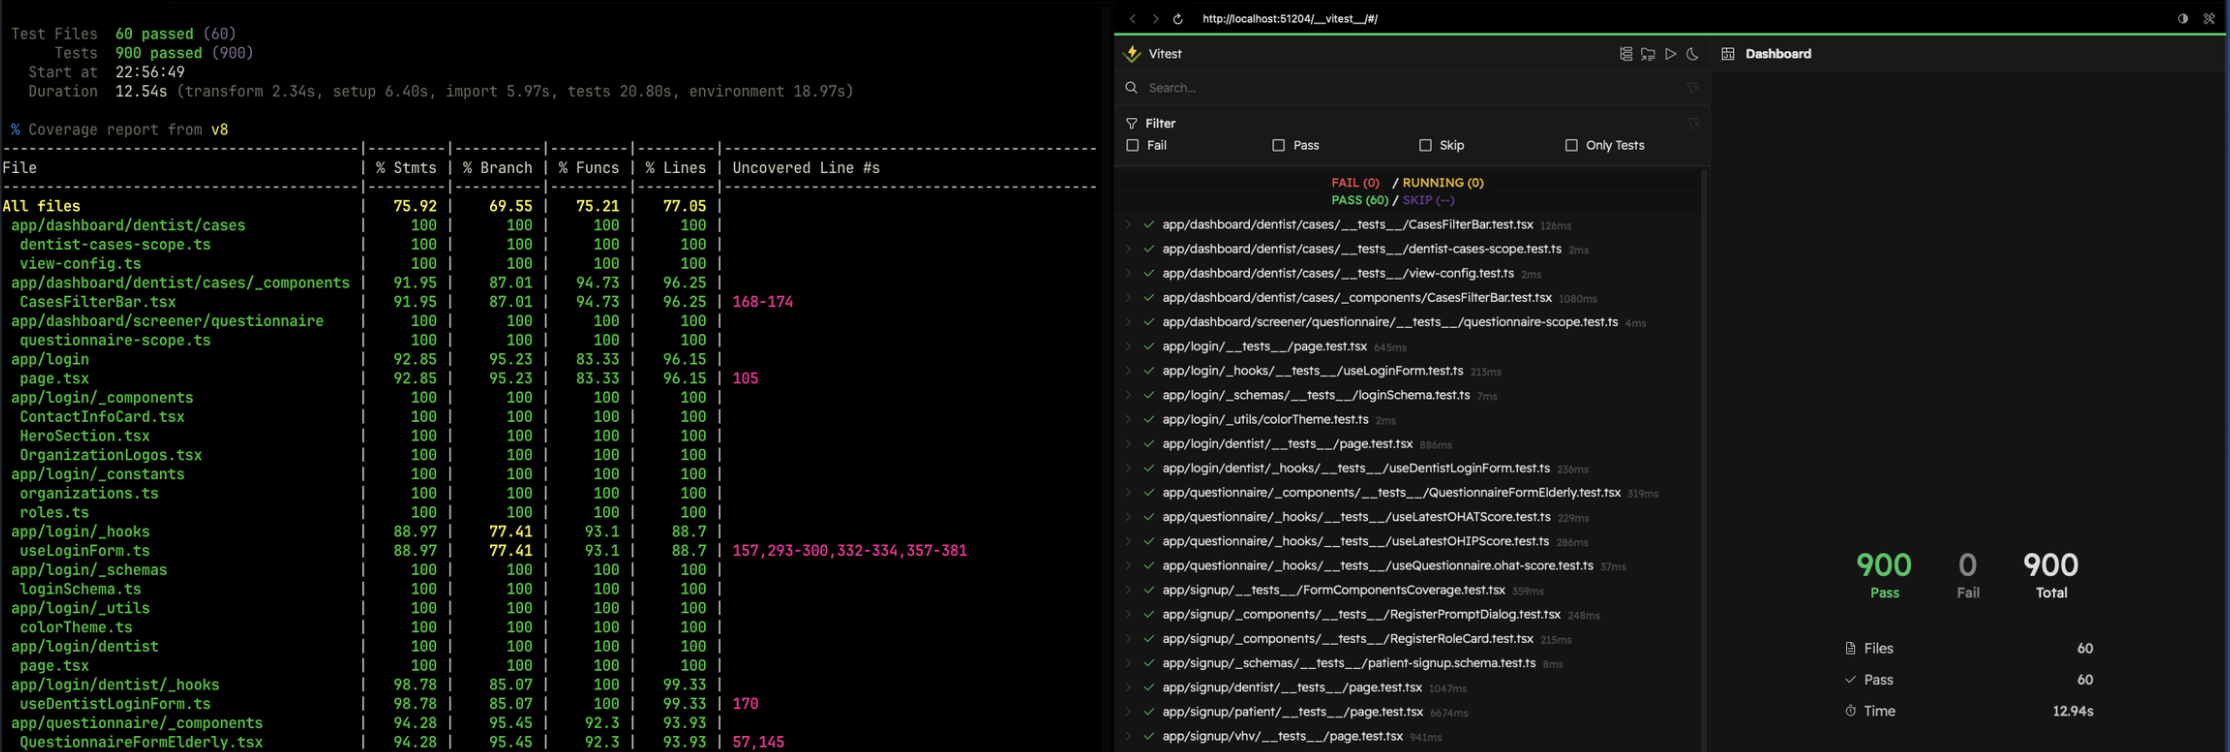
\includegraphics[width=\linewidth]{images/4.1.2.png}
  \caption{ผลการทดสอบ Unit/Integration: Coverage Report และ Vitest UI
    (900 passed, 0 failed) โดยรันเสร็จภายใน $<13\,\text{s}$}
\end{figure}

\begin{tcolorbox}[greenbox]
  \renewcommand{\arraystretch}{1.4}
  \begin{tabularx}{\linewidth}{Xl}
    \textbf{จำนวน Test ทั้งหมด} & 900 (Unit + Integration)\\
    \textbf{สถานะ} & \textcolor{successgreen}{\textbf{ผ่าน 100\%}}\\
    \textbf{Code Coverage} & $\approx$75\%\\
    \textbf{Critical Logic} & \textbf{100\%}\\
    \textbf{เวลาในการทดสอบ} & $<13\,\text{s}$\\
  \end{tabularx}
\end{tcolorbox}

% =========================
\subsection{โปรไฟล์ภาระงานสังเคราะห์ (Synthetic Load)}

\begin{tcolorbox}[bluebox,title={สรุปผล Synthetic Load}]
  \renewcommand{\arraystretch}{1.35}
  \begin{tabularx}{\linewidth}{Xl}
    \textbf{ระยะเวลา} & 1 ชั่วโมง\\
    \textbf{จำนวน Request} & 7,632\\
    \textbf{ค่าเฉลี่ย RPS} & 2.12\\
    \textbf{Success Rate} & 99.46\%\\
  \end{tabularx}
\end{tcolorbox}

\begin{figure}[H]
  \centering
  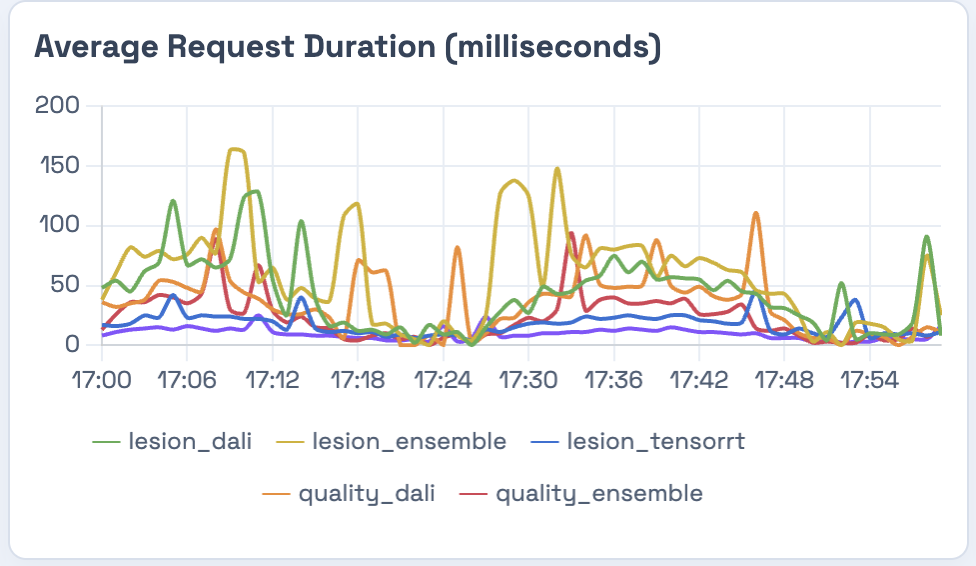
\includegraphics[width=\linewidth]{images/4.1.png}
  \caption{Request Duration}
\end{figure}

\begin{figure}[H]
  \centering
  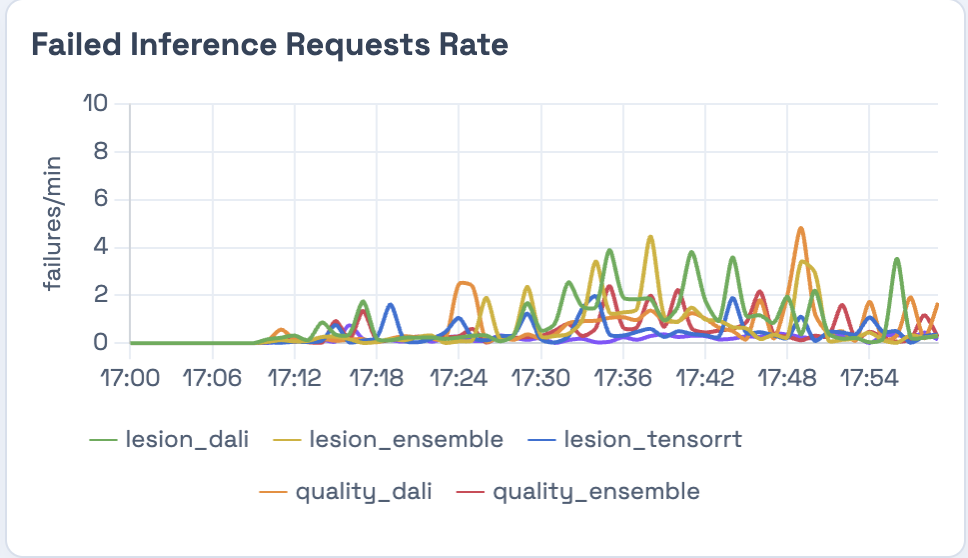
\includegraphics[width=\linewidth]{images/4.2.png}
  \caption{Failed Requests}
\end{figure}

\begin{figure}[H]
  \centering
  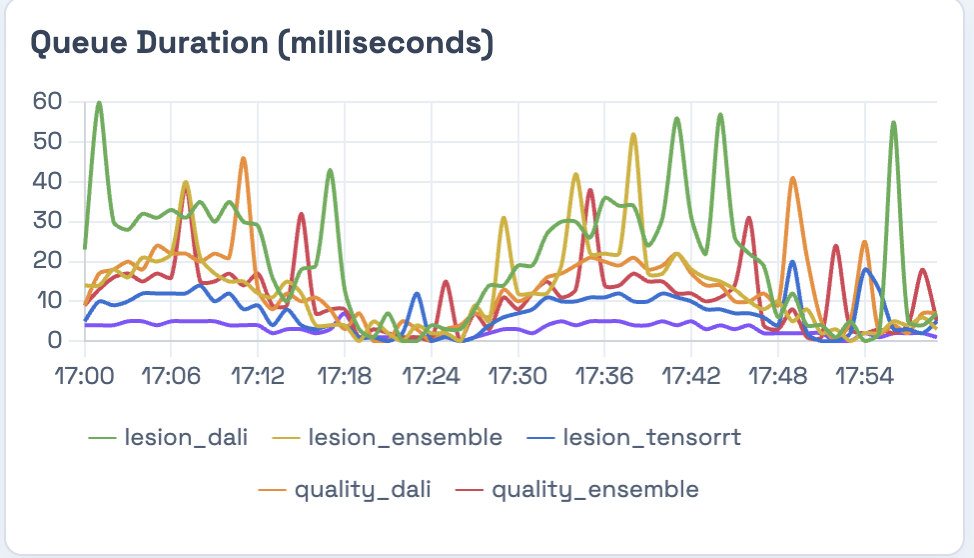
\includegraphics[width=\linewidth]{images/4.3.png}
  \caption{Queue Time}
\end{figure}

\begin{figure}[H]
  \centering
  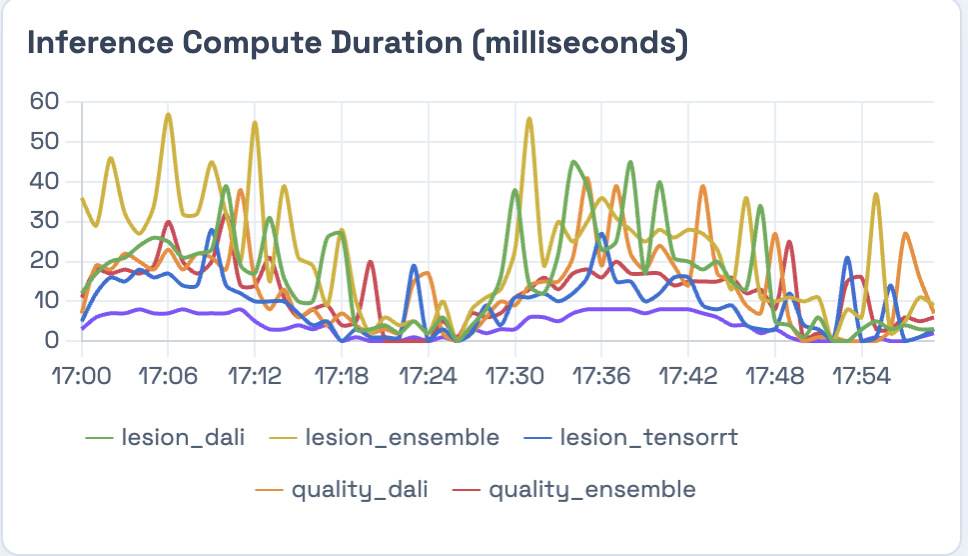
\includegraphics[width=\linewidth]{images/4.4.png}
  \caption{Compute Time}
\end{figure}

\begin{figure}[H]
  \centering
  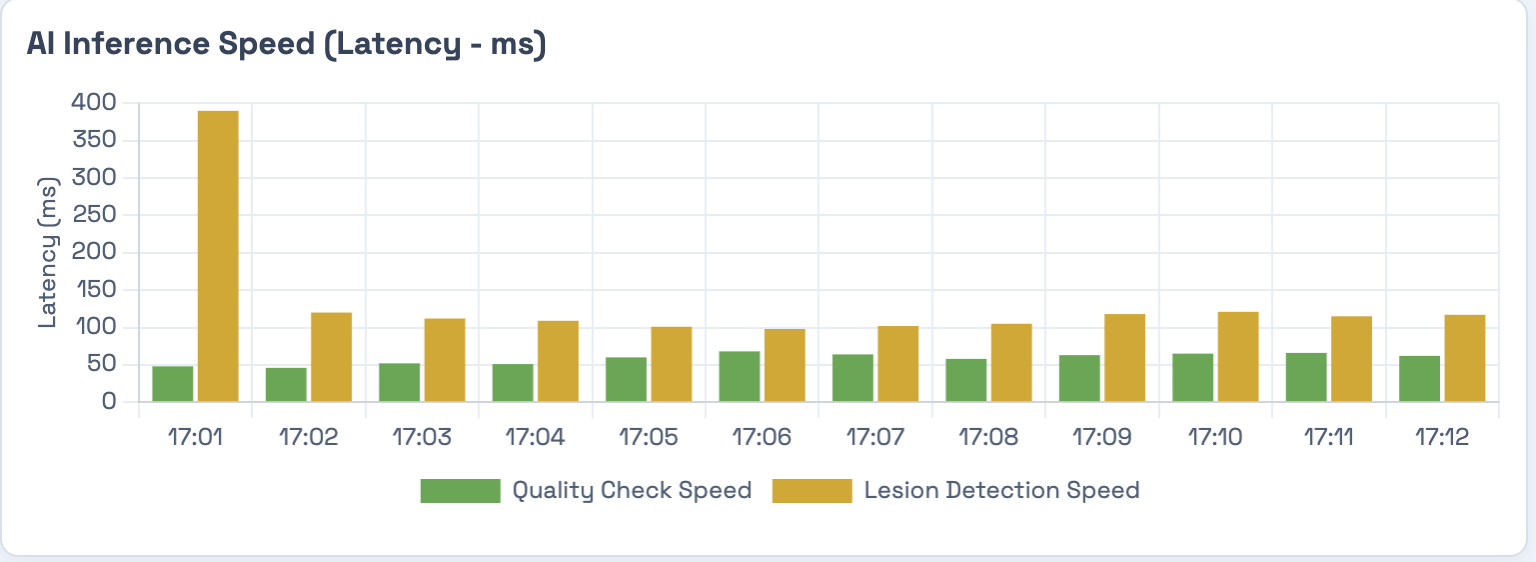
\includegraphics[width=\linewidth]{images/4.5.png}
  \caption{AI Inference Latency}
\end{figure}

% =========================
\subsection{การวิเคราะห์ผลการทดสอบ}

จากผลการทดสอบพบว่า ระบบมีอัตราความสำเร็จสูงถึง 99.46\% ซึ่งสะท้อนถึงความเสถียรภายใต้ภาระงานต่อเนื่อง

แม้ค่า RPS จะไม่สูงมาก แต่สอดคล้องกับลักษณะการใช้งานจริงในระดับชุมชน ซึ่งไม่ได้มีรูปแบบการใช้งานหนาแน่นเช่นระบบขนาดใหญ่

นอกจากนี้ ค่า latency และ queue time ที่ต่ำ แสดงให้เห็นว่าระบบสามารถจัดการคำขอได้อย่างมีประสิทธิภาพ และไม่เกิด bottleneck ใน pipeline

% =========================
\section{การอภิปรายผล}

จากผลการทดสอบพบว่า ความสำเร็จของระบบไม่ได้ขึ้นอยู่กับ AI เพียงอย่างเดียว แต่เกิดจากการออกแบบระบบโดยรวม ทั้งด้านสถาปัตยกรรม workflow และ usability

การใช้ Modular Monolith Architecture และ Dual-Path AI ช่วยเพิ่มความเสถียรและลดความเสี่ยงจากการล่มของระบบ ซึ่งเป็นปัจจัยสำคัญในระบบทางการแพทย์

นอกจากนี้ การออกแบบ workflow ให้สอดคล้องกับการทำงานจริงของบุคลากร เช่น อสม. และทันตแพทย์ มีบทบาทสำคัญในการทำให้ระบบสามารถใช้งานจริงได้

อย่างไรก็ตาม ยังมีข้อจำกัด เช่น การพึ่งพา AI จากภายนอก และการทดสอบที่ยังอยู่ในระดับนำร่อง

% =========================
\section{สรุปผลการดำเนินงาน}

ระบบ eDENT-ELDER Phase 2 สามารถทำงานได้ครบถ้วนตามวัตถุประสงค์ และมีศักยภาพในการนำไปใช้งานจริง

ระบบสามารถเพิ่มการเข้าถึงบริการ ลดภาระของบุคลากร และเพิ่มประสิทธิภาพในการตรวจพบโรคในระยะเริ่มต้น

ผลการทดสอบทั้งด้าน functional และ performance ยืนยันถึงความพร้อมของระบบสำหรับการใช้งานจริงในระดับบริการ
\chapter{\ifenglish Conclusion\else บทสรุป\fi}

\section{สรุปและบทสรุป}


โครงการ eDENT-ELDER Phase 2 มีเป้าหมายเพื่อแก้ไขข้อจำกัดของระบบเดิม
และพัฒนาแพลตฟอร์มสำหรับการคัดกรองมะเร็งช่องปากในระดับชุมชนให้สามารถใช้งานได้จริง

จากผลการดำเนินงานในบทก่อนหน้า พบว่าระบบสามารถรองรับกระบวนการคัดกรองแบบครบวงจร
ตั้งแต่การเก็บข้อมูลผู้ป่วย การวิเคราะห์ด้วย AI ไปจนถึงการให้คำปรึกษาจากผู้เชี่ยวชาญ
โดยมีความเสถียรและประสิทธิภาพในระดับที่เหมาะสมต่อการใช้งานจริง

นอกจากนี้ การออกแบบระบบในลักษณะ Modular Monolith architecture
ร่วมกับแนวคิด Dual-Path AI และ DevOps Pipeline
ช่วยให้ระบบมีความยืดหยุ่น สามารถขยายระบบได้ในอนาคต
และลดความเสี่ยงจากความล้มเหลวของระบบ

\begin{tcolorbox}[bluebox, title=ผลสำเร็จหลัก]
  \begin{itemize}[leftmargin=1.4em, itemsep=5pt]
    \item \textbf{สถาปัตยกรรม:}
          Modular Monolith architecture (Next.js + FastAPI + DDD) แทนสถาปัตยกรรมเดิมแบบ monolith
    \item \textbf{ระบบ AI:}
          Dual-Path AI มี inference latency $<200\,\text{ms}$ ภายใต้ synthetic load
          อัตรา request สำเร็จ 99.46\% จากทั้งหมด 7,632 requests
    \item \textbf{ความปลอดภัย:}
          กรอบ PDPA/HIPAA พร้อม Tamper-Proof Audit Logging
          และ Role-Based Access Control (RBAC) ครอบคลุม 6 บทบาท
    \item \textbf{DevOps:}
          Docker Containerization ครบวงจร พร้อม CI/CD Pipeline
          และการแยก Environment เข้มงวด
    \item \textbf{คุณภาพ:}
          900 automated tests ผ่าน 100\%
          100\% coverage บน critical business logic
    \item \textbf{ความร่วมมือ:}
          หลายสถาบัน ครอบคลุมทันตแพทยศาสตร์ วิศวกรรมศาสตร์ และสาธารณสุขชุมชน
  \end{itemize}
\end{tcolorbox}

แพลตฟอร์มพร้อม Deploy ระดับนำร่องในเชียงใหม่ พะเยา ภูเก็ต และหนองบัวลำภู
เพื่อช่วยให้ตรวจพบมะเร็งช่องปากในผู้สูงอายุชนบทเร็วขึ้น
ลดการวินิจฉัยระยะท้าย และพัฒนาผลลัพธ์ผู้ป่วยในวงกว้าง

โครงการนี้ประสบความสำเร็จในการแก้ปัญหาคอขวดและจุดล้มเหลวของระบบเดิม
เปลี่ยนผ่านสู่ \textbf{แพลตฟอร์มทางการแพทย์พร้อมใช้งานจริง (Production-Ready)}
ด้วยสถาปัตยกรรมที่เสถียร ปลอดภัย และเหมาะสมต่อการใช้งานจริงในระดับบริการ
\vspace{0.5em}
\begin{tcolorbox}[graybox]
  \textbf{ข้อจำกัดของโครงการ (Limitations):}
  \begin{itemize}[leftmargin=1.4em, itemsep=3pt]
    \item ระบบพึ่งพา AI Model จากภายนอก
          ซึ่งอาจมีข้อจำกัดด้านการควบคุมคุณภาพและการปรับปรุงโมเดล
    \item การทดสอบยังอยู่ในระดับนำร่อง
          และยังไม่ได้ประเมินผลในระดับประชากรขนาดใหญ่
    \item ประสิทธิภาพของระบบขึ้นอยู่กับคุณภาพของภาพที่ผู้ใช้งานส่งเข้ามา
    \item การยอมรับของผู้ใช้งานในระยะยาวยังต้องมีการศึกษาเพิ่มเติม
  \end{itemize}
\end{tcolorbox}
\vspace{0.5em}
\begin{tcolorbox}[graybox]
  \textbf{งานในอนาคต (Future Work):}
  \begin{itemize}[leftmargin=1.4em, itemsep=3pt]
    \item ขยาย AI Model ครอบคลุมรอยโรคช่องปากเพิ่มเติม
          และปรับปรุงความแม่นยำด้วย Dataset Annotation จากพื้นที่นำร่อง
    \item ขยายสู่จังหวัดเพิ่มเติมและเชื่อมต่อกับระบบสารสนเทศสุขภาพ (HIS) ของไทย
    \item ดำเนินการศึกษา Clinical Validation อย่างเป็นทางการ
          วัด Stage-Shift และเวลาพบผู้เชี่ยวชาญในกลุ่มนำร่อง
    \item สำรวจการเชื่อมต่อ LINE OA และ PWA Offline Mode
          สำหรับชุมชนที่มีอินเทอร์เน็ตจำกัด
  \end{itemize}
\end{tcolorbox}
\vspace{0.5em}
โดยสรุป โครงการนี้แสดงให้เห็นถึงศักยภาพของการผสานเทคโนโลยีดิจิทัล
เข้ากับระบบสาธารณสุขในระดับชุมชนอย่างเป็นรูปธรรม
และสามารถต่อยอดสู่การใช้งานในระดับประเทศได้ในอนาคต
\vfill
{\color{primaryblue}\rule{\linewidth}{1pt}}
\begin{center}
  \small\color{medgray}
  eDENT-ELDER เฟส 2 รายงานโครงงานฉบับสมบูรณ์ $\cdot$
  รหัสวิชา 261492 $\times$ 2568 $\cdot$
  ภาควิชาวิศวกรรมคอมพิวเตอร์ คณะวิศวกรรมศาสตร์ มหาวิทยาลัยเชียงใหม่
\end{center}

\appendix
\chapter{\ifenglish Appendix\else ภาคผนวก\fi}

% =====================================================
\section{\ifenglish End-to-End System Execution\else การทำงานของระบบแบบครบวงจร (Real Execution)\fi}

แสดงการทำงานจริงของระบบตั้งแต่ต้นจนจบ

\begin{itemize}
  \item Login → Register → Consent → Workflow → Diagnosis
  \item การไหลของข้อมูลจริงในระบบ
\end{itemize}

📌 \textbf{[ใส่รูป]} Full real workflow (step-by-step screenshots)

% =====================================================
\section{\ifenglish Authentication and User Management\else ระบบยืนยันตัวตนและจัดการผู้ใช้งาน\fi}

\subsection*{Login Flow}
\begin{itemize}
  \item กรอกเบอร์โทร
  \item รับ OTP
  \item ยืนยันตัวตน
\end{itemize}

📌 \textbf{[ใส่รูป]} Login UI + OTP screen

\subsection*{Register and Consent}
\begin{itemize}
  \item ลงทะเบียนผู้ใช้ใหม่
  \item ยอมรับ PDPA Consent
\end{itemize}

📌 \textbf{[ใส่รูป]} Register + Consent screen

\subsection*{Role Assignment}
\begin{itemize}
  \item Patient
  \item VHV (อสม.)
  \item Screener
  \item Specialist
\end{itemize}

📌 \textbf{[ใส่รูป]} Role selection / dashboard แตกต่างกัน

% =====================================================
\section{\ifenglish Patient and VHV Workflow\else การใช้งานของผู้ป่วยและ อสม.\fi}

\begin{enumerate}
\item เลือกผู้ป่วย
\item กรอกข้อมูล
\item ทำแบบประเมิน OHAT / OHIP
\item ถ่ายภาพช่องปาก
\item ส่งข้อมูลเข้า AI
\end{enumerate}

📌 \textbf{[ใส่รูป]} ทุก step แบบ sequence

% =====================================================
\section{\ifenglish AI Processing and Results\else การประมวลผล AI และผลลัพธ์\fi}

\begin{itemize}
  \item ภาพ input จริง
  \item ผล AI (classification / detection)
  \item confidence score
\end{itemize}

📌 \textbf{[ใส่รูป]} Before / After AI

% =====================================================
\section{\ifenglish Screener Workflow\else การทำงานของผู้คัดกรอง\fi}

\begin{enumerate}
\item ดูรายการเคส
\item วิเคราะห์ผล AI
\item ตัดสินใจส่งต่อ
\end{enumerate}

📌 \textbf{[ใส่รูป]} Screener dashboard + case detail

% =====================================================
\section{\ifenglish Specialist Workflow\else การทำงานของผู้เชี่ยวชาญ\fi}

\begin{enumerate}
\item รับเคส referral
\item ตรวจสอบภาพและข้อมูล
\item วินิจฉัย
\item ปิดเคส
\end{enumerate}

📌 \textbf{[ใส่รูป]} Specialist dashboard

% =====================================================
\section{\ifenglish API and Data Exchange\else การสื่อสารข้อมูลและ API\fi}

\subsection*{Authentication API}
\begin{verbatim}
POST /api/auth/otp
\end{verbatim}

\subsection*{Inference API}
\begin{verbatim}
POST /api/inference
\end{verbatim}

\subsection*{Response Example}
\begin{verbatim}
{
  "risk": "high",
  "confidence": 0.91
}
\end{verbatim}

% =====================================================
\section{\ifenglish Database Structure\else โครงสร้างฐานข้อมูล\fi}

\begin{itemize}
  \item Patient table
  \item Case table
  \item AI result table
\end{itemize}

📌 \textbf{[ใส่รูป]} ER Diagram จริง

% =====================================================
\section{\ifenglish DevOps and Deployment Evidence\else หลักฐาน DevOps และการ Deploy\fi}

\begin{itemize}
  \item Docker container
  \item CI/CD pipeline
  \item Deployment logs
\end{itemize}

📌 \textbf{[ใส่รูป]} Pipeline / logs

% =====================================================
\section{\ifenglish Testing Evidence\else หลักฐานการทดสอบระบบ\fi}

\begin{itemize}
  \item Unit test (Vitest)
  \item Coverage report
  \item Load test (Grafana)
\end{itemize}

📌 \textbf{[ใส่รูป]} Test results

% =====================================================
\section{\ifenglish Security Implementation\else การออกแบบความปลอดภัย\fi}

\begin{itemize}
  \item JWT Flow
  \item RBAC
  \item Encryption
\end{itemize}

📌 \textbf{[ใส่รูป]} Security diagram / flow

% =====================================================
\section{\ifenglish System Manual\else คู่มือการใช้งานระบบ\fi}

\subsection*{Patient / VHV}
\begin{enumerate}
\item Login
\item กรอกข้อมูล
\item ถ่ายภาพ
\item รับผล
\end{enumerate}

\subsection*{Screener}
\begin{enumerate}
\item ตรวจเคส
\item วิเคราะห์
\item ส่งต่อ
\end{enumerate}

\subsection*{Specialist}
\begin{enumerate}
\item รับเคส
\item วินิจฉัย
\item ปิดเคส
\end{enumerate}

\end{document}
